%%%%%%%%%%%%%%%%%%%%%%%%%%%%%%%%%%%%%%%%%
% Academic Title Page
% LaTeX Template
% Version 2.0 (17/7/17)
%
% This template was downloaded from:
% http://www.LaTeXTemplates.com
%
% Original author:
% WikiBooks (LaTeX - Title Creation) with modifications by:
% Vel (vel@latextemplates.com)
%
% License:
% CC BY-NC-SA 3.0 (http://creativecommons.org/licenses/by-nc-sa/3.0/)
%
% Instructions for using this template:
% This title page is capable of being compiled as is. This is not useful for
% including it in another document. To do this, you have two options:
%
% 1) Copy/paste everything between \begin{document} and \end{document}
% starting at \begin{titlepage} and paste this into another LaTeX file where you
% want your title page.
% OR
% 2) Remove everything outside the \begin{titlepage} and \end{titlepage}, rename
% this file and move it to the same directory as the LaTeX file you wish to add it to.
% Then add \input{./<new filename>.tex} to your LaTeX file where you want your
% title page.
%
%%%%%%%%%%%%%%%%%%%%%%%%%%%%%%%%%%%%%%%%%

%----------------------------------------------------------------------------------------
%	PACKAGES AND OTHER DOCUMENT CONFIGURATIONS
%----------------------------------------------------------------------------------------

\documentclass[11pt]{article}

\usepackage[a4paper, margin={2cm, 3cm}]{geometry}

\usepackage{multicol}

\usepackage[utf8]{inputenc} % Required for inputting international characters
\usepackage[T1]{fontenc} % Output font encoding for international characters

\usepackage{mathpazo} % Palatino font

\usepackage[english]{babel}
\usepackage{csquotes}

\usepackage{fancyhdr}
\pagestyle{fancy}
\fancyhf{}
\rhead{D.J. Holland}
\lhead{ICT40010 — Technical Report}
\rfoot{\thepage}

\usepackage[toc,page]{appendix}

\usepackage[
  backend=biber,
]{biblatex}
\addbibresource{../../ICT40010.bib}

\usepackage{graphicx}

\usepackage{minted}
\usemintedstyle{manni}
\newminted{rust}{
  autogobble,
  bgcolor=gray!10,
  fontsize=\footnotesize,
  samepage,
}
\newmintinline{rust}{bgcolor=gray!10}
\def\rust{\rustinline}
\newmintinline{text}{bgcolor=gray!10}
\def\code{\textinline}

\usepackage[dvipsnames]{xcolor}
\definecolor{FuchsiaPink}{HTML}{af30ed}
\definecolor{ScooterBlue}{HTML}{30c9ed}

\usepackage{hyperref}
\hypersetup{
    colorlinks=true,
    allcolors=FuchsiaPink,
}

\usepackage{fontspec}
\newfontface\emojifont{Twitter Color Emoji}
\newcommand{\emoji}[1]{{\emojifont{#1}}}

\begin{document}


%----------------------------------------------------------------------------------------
%	TITLE PAGE
%----------------------------------------------------------------------------------------

\begin{titlepage} % Suppresses displaying the page number on the title page and the subsequent page counts as page 1
  \newcommand{\HRule}{\rule{\linewidth}{0.5mm}} % Defines a new command for horizontal lines, change thickness here

  \center{} % Centre everything on the page

  %------------------------------------------------
  %	Headings
  %------------------------------------------------

  % Main heading such as the name of your university/college
  \textsc{\LARGE Swinburne University of Technology}\\[1.5cm]

  % Major heading such as course name
  \textsc{
    \Large
    Bachelor of Engineering\\
    (Software Engineering)\\
    (Honours)
  }\\[0.5cm]

  % Minor heading such as course title
  \textsc{\large ICT40010 Research Report A}\\[0.5cm]

  %------------------------------------------------
  %	Title
  %------------------------------------------------

  \HRule{}\\[0.4cm]

  % Title of your document
  {\huge\bfseries Technical Report}\\[0.2cm]

  \HRule{}\\[1.5cm]

  %------------------------------------------------
  %	Author(s)
  %------------------------------------------------

  \begin{minipage}{0.4\textwidth}
    \begin{flushleft}
      \large
      \textit{Author}\\
      D.J. \textsc{Holland}
    \end{flushleft}
  \end{minipage}
  {~}
  \begin{minipage}{0.4\textwidth}
    \begin{flushright}
      \large
      \textit{Supervisors}\\
      Dr.\ Clinton \textsc{Woodward}\\
      Dr.\ Charlotte \textsc{Pierce}
    \end{flushright}
  \end{minipage}

  % If you don't want a supervisor, uncomment the two lines below and comment the code above
  %{\large\textit{Author}}\\
  %John \textsc{Smith} % Your name

  %------------------------------------------------
  %	Date
  %------------------------------------------------

  \vfill\vfill\vfill % Position the date 3/4 down the remaining page

  {\large\today} % Date, change the \today to a set date if you want to be precise

  %------------------------------------------------
  %	Logo
  %------------------------------------------------

  \vfill\vfill
  
\includegraphics[width=0.2\textwidth]{../swin-logo.jpg}\\[1cm] % Include a department/university logo - this will require the graphicx package

  %----------------------------------------------------------------------------------------

  % \vfill % Push the date up 1/4 of the remaining page

\end{titlepage}

%----------------------------------------------------------------------------------------
%	ABSTRACT
%----------------------------------------------------------------------------------------

\pagenumbering{gobble}

% Add an abstract (answer context, gap, method, outcomes, implications question.)
\begin{abstract}
  In real-time computer graphics, a rendering pipeline provides a workflow to draw things on the screen.
  There are two contemporary methods to visualise geometry and shading, Forward Rendering and Deferred Rendering.
  This paper specifies the technical details of implementing such rendering pipelines.
  Using the Rust programming language for its performance and OpenGL as the definitive cross-platform graphics API, an application was created to benchmark the performance of the two rendering pipelines to determine which pipeline best suits what general usage scenarios.
\end{abstract}

\newpage

%----------------------------------------------------------------------------------------
%	CONTENTS
%----------------------------------------------------------------------------------------

\tableofcontents
% \pagenumbering{gobble}
\newpage
\pagenumbering{arabic}

%----------------------------------------------------------------------------------------
%	REPORT
%----------------------------------------------------------------------------------------

\section{Introduction}
% Add Intro - should be pretty easy - it’s the abstract again but with more context/gap if you need too and a final blurb about the structure of the report. i.e. “In Section 2 … then Section 3 presents ….. “
3D applications, such as video games, require efficient and approximate visualising of scene data; rendering geometry and shading it.
Forward Rendering and Deferred Rendering are the two main ways to accomplish this.
Forward Rendering draws and shades each fragment of each object, even if that pixel does not end up in the final image.
Deferred rendering rasterises all the geometry data in the scene before doing shading calculations to avoid shading fragments that will not be visible.
This paper contains implementation details for an application capable of comparing both pipelines.

In Section~\ref{sec:technology} and Section~\ref{sec:foundation} of this paper, the technology stack for the application is discussed.
Section~\ref{sec:architecture} covers the overall architecture of the software, and Section~\ref{sec:main-loop} goes over the main event loop.
In Section~\ref{sec:renderer}, details on the rendering pipeline implementations are specified.

% \begin{multicols}{2}

\section{Technology}\label{sec:technology}
% Break “Technology” sections into groups - suggest primary (required) and supporting (VS Code GitHub) or similar. Then also do an “intro” section to explain the groups of technology used. Code snippets are fine here in this section. Remember, purpose of tech report is to help someone like yourself reproduce the apparatus/setup to be able to do what you have done, and to also understand why you have made the choice you have (so that they could modify as appropriate).

\subsection{Introduction}
The primary technologies used in the application are Rust and OpenGL\@.
Several supporting technologies were used to aid the development, including, Visual Studio Code and GitHub.

\subsection{Primary}

\paragraph{\emoji{🦀} Rust.}
Rust is a systems programming language that guarantees memory safety at compile time.
Rust does not need a garbage collector so the performance is excellent with little to no overhead.
There is zero-cost bidirectional interoperability with C via the FFI\@;
a basic requirement for communicating with OpenGL on the system~\autocite{rust_programming_language_rust_2020}.

The modern Rust tool-chain makes it trivial to have a fast and friendly developer experience.

\paragraph{OpenGL.}
The OpenGL API is a standard in high-performance cross-platform graphics, with a wealth of learning resources available.
Using OpenGL and Rust enables the application to run on Windows, macOS, and Linux without much platform specific thought. OpenGL \textinline{4.1} is minimum target version as that is the latest version supported on macOS \autocite{opengl_opengl_2020}.

Vulkan was considered, but due to the increased complexity of properly implementing a Vulkan based application, OpenGL was the simpler choice \autocite{vulkan_vulkan_2020}.

\subsection{Supporting}

\paragraph{Visual Studio Code.}
Continuing with cross-platform tools, VS Code is the text-editor/IDE of choice \autocite{visual_studio_code_visual_2020}.
Using the excellent rust-analyzer extension, it is a decent Rust IDE\@.
With various other extensions, writing shader code and documentation is also pleasant.

\paragraph{GitHub.}
Several services on GitHub are used:
\begin{itemize}
  \item It is the main git remote repository for the source code
  \item Issues can be tracked there
  \item Projects, labels, and milestones help triage those issues
  \item Actions are used to build and test the code (CI)
  \item Pages is used to host the project website which is deployed from Actions (CD).
\end{itemize}
\autocite{github_github_2020}

\paragraph{VuePress.}
VuePress is a static site generator particularly designed for writing technical documentation \autocite{vuepress_vuepress_2020}.
It is used to generate the projet website.

\section{Foundation}\label{sec:foundation}

\subsection{Crates}
Rust's package manager, \textbf{Cargo}, allows code dependencies to be easily required by specifying them in a \code{Cargo.toml} file.
In “Rust-land”, packages are known as \textbf{Crates}.

Many crates are used in the application, with the most fundamental ones being outlined below.

\subsection{\code{gl}}
Unsafe bindings to raw OpenGL calls.
This is what allows the application to interoperate with OpenGL on the system.
If this crate did not exist, then this application would have been written with C++ because generating function pointers for system APIs is not within the scope this project.

\subsection{\code{glutin}}
Manages windowing, events, and the OpenGL context.
Another excellent create for cross-platform windowing and IO\@.
The functions from the \code{gl} crate get loaded by the OpenGL context that \code{glutin} creates.

\subsection{\code{imgui}}
Immediate Mode Graphical User Interface.
Creating UI is out of the scope of this project, IMGUI is an incredibly popular rendering-API-agnostic library for creating development tooling.
This crate provides some safe abstraction as well as bindings to every IMGUI function.

\subsection{\code{nalgebra-glm}}
This crate is a subset of linear algebra tools from the \code{nalgebra} crate specifically for mathematics used in graphics programming.

\section{Architecture}\label{sec:architecture}

\subsection{Modules}
Rust's module system provides an easy way to group code for readability, reuse, and privacy.
The boxes in Figure~\ref{fig:module-graph} are derivative of the directory structure of the source code, with important modules having further explanation following.

The application is split into two main projects:
\begin{itemize}
  \item \textbf{Sandbox}: A binary application to run and demonstrate the Glamour library.
  \item \textbf{Glamour}: A library project containing all the rendering functionality.
\end{itemize}

\begin{figure}
  \begin{center}
    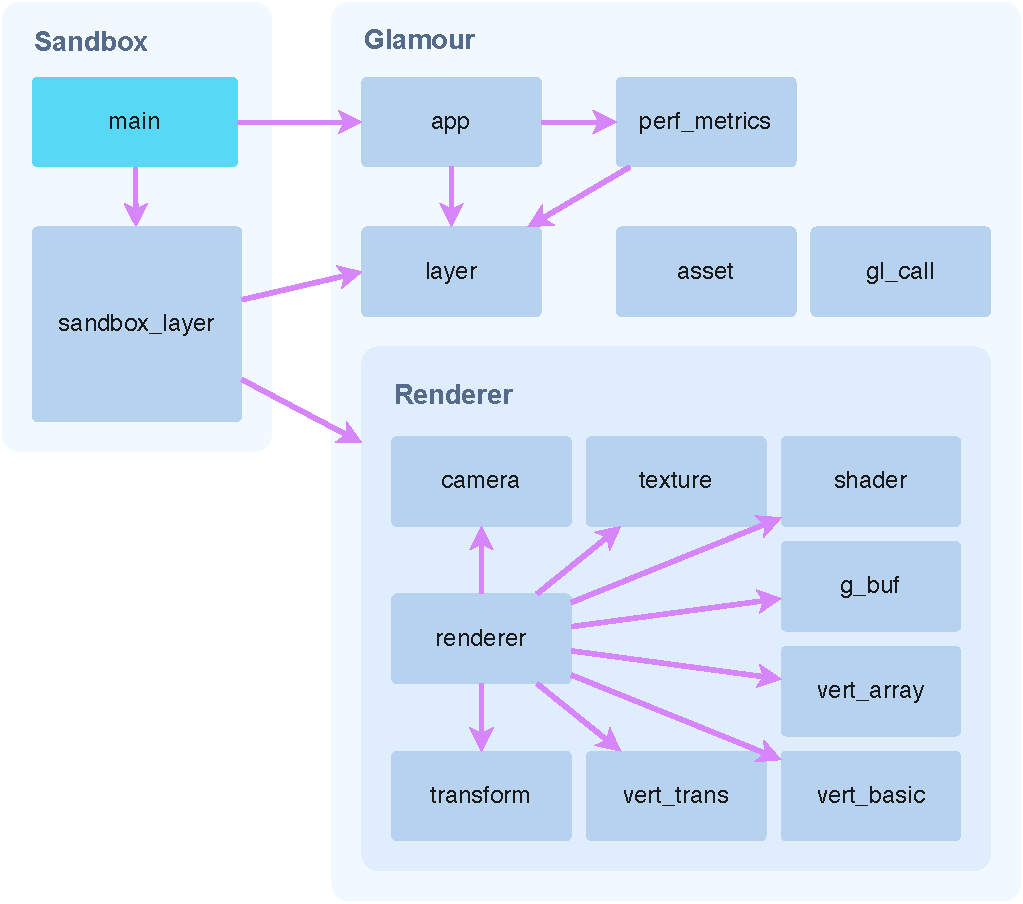
\includegraphics[width=0.7\columnwidth]{../module-graph.pdf}
  \end{center}
  \caption[Module graph]{\emph{A simplified module and dependency graph for the application.}}\label{fig:module-graph}
\end{figure}

\paragraph{\code{app}}
The app module is responsible for managing the window, event loop, and OpenGL context.
This is where layers are stored and processed.

\paragraph{\code{layer}}
A layer is a trait (like an interface) that can handle events and do things on update loops.

\paragraph{\code{asset}}
This module provides a way to load files from the \code{assets} folder, which is copied relative to the executable on build.

\paragraph{\code{gl_call}}
Since all the OpenGL functions are inherently \emph{unsafe}, the \code{gl_call!} macro will wrap a function and \emph{panic} if it errors, making OpenGL much easier to use.

\paragraph{\code{renderer}}
This is what actually makes the draw calls.
The renderer also manages the shaders, vertex arrays, and G-buffer, amongst other things.

\subsection{Sandbox}
The Sandbox project initialises an \code{app} instance and attaches a \code{sandbox_layer} to it.
The \code{sandbox_layer} is responsible for instructing the \code{renderer} what to render, e.g., \emph{render 10,000 cubes at these randomly seeded positions from this camera angle}.

\section{Main Loop}\label{sec:main-loop}

\subsection{Initialising}
The \code{main} function in Sandbox only contains four lines. See Appendix~\ref{app:sandbox-main}.
Calling the \code{new} function\footnote{\rust{glamour::App::new(title: &str, width: u32, height: u32)}} will do the following:
\begin{itemize}
  \item Create a new event loop from the \code{glutin} crate to handle OS I/O
  \item Build a window with the supplied \code{title}, \code{width}, and \code{height}
  \item Load OpenGL within that window's context
  \item Load imgui
  \item Initialise the Layer stack.
\end{itemize}
After this point, layers can be pushed to the app, and then run.

\subsection{Layer}
A \code{Layer} is a basic trait to handle events of distinct parts of the application.
Layers do not communicate with each other through the app, they are meant to be separate.
There are only two layers used in the app:
\begin{itemize}
  \item \code{PerfMetricsLayer} for reporting performance metrics
  \item \code{SandboxLayer} is a place to store all Sandbox related things.
\end{itemize}
\code{Layer} provides a few functions that an implementation can use:
\begin{itemize}
  \item \code{init()}
  \item \code{on_event()}
  \item \code{on_fixed_update()}
  \item \code{on_frame_update()}
  \item \code{on_imgui_update()}
\end{itemize}

Hopefully, those should be fairly self documenting.

\subsection{Event Loop}
Calling \code{app.run()} kick-starts the main event loop, which is responsible for
\begin{itemize}
  \item Polling for events
  \item Managing fixed and frame updates
  \item Updating and rendering imgui
  \item Calling each layer's \code{Layer} trait functions at the appropriate point
  \item Swapping the frame buffer to actually show the rendered image on the screen.
\end{itemize}

\subsection{AppContext}
\code{App} also maintains a struct that holds the context of the application.
This is \code{AppContext}, it provides some convenience to access things such as the window context and frame timings.
This is passed to each \code{Layer} function.

\section{Renderer}\label{sec:renderer}

% TODO: Details on the rendering pipeline, how OpenGL is used, and performance metrics.
% use lots of pictures here, it is the main visual element.

\subsection{Pipeline}

\subsubsection{Overview}

\begin{figure}
  \begin{center}
    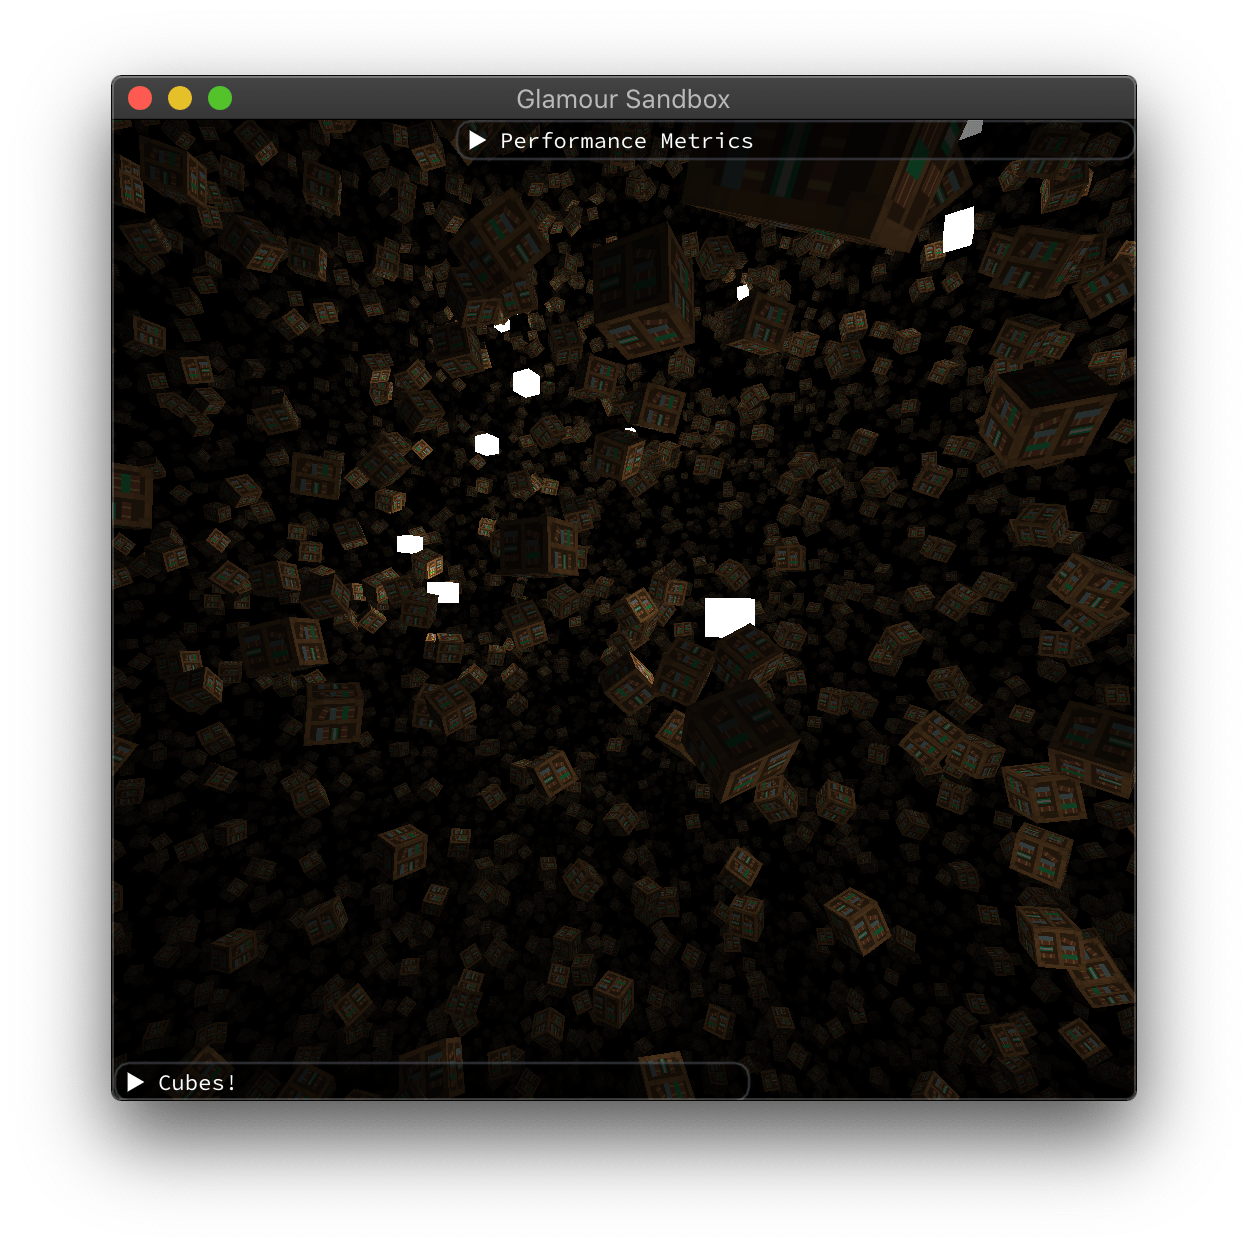
\includegraphics[width=0.6\columnwidth]{../sandbox.png}
  \end{center}
  \caption[Sandbox screenshot]{
    \emph{
      Running the application results in the scene above.
      A bunch of rotating textured cubes, with lights travelling around the world.
    }
  }\label{fig:sandbox-screenshot}
\end{figure}

In the main event loop, when a draw is requested (either by the OS or when the frame update timer is done), \code{on_frame_update()} is called for each Layer.
This layer hook is generally where interaction with the Renderer should happen, and pipeline start and end before the frame buffers are swapped.

To draw the scene in Figure~\ref{fig:sandbox-screenshot}, the Sandbox application follows the pipeline visualised in Figure~\ref{fig:rendering-pipeline}.
The pipeline is the same for forward rendering and deferred rendering, with the difference being in how the entities (the cubes) are drawn and shaded in the \textbf{End Draw} phase.

\textbf{Begin Draw}, \textbf{Update Entities}, and \textbf{Update Lights} all function to transform and send data to the GPU before drawing, which actually happens in \textbf{End Draw}.

\begin{figure}
  \begin{center}
    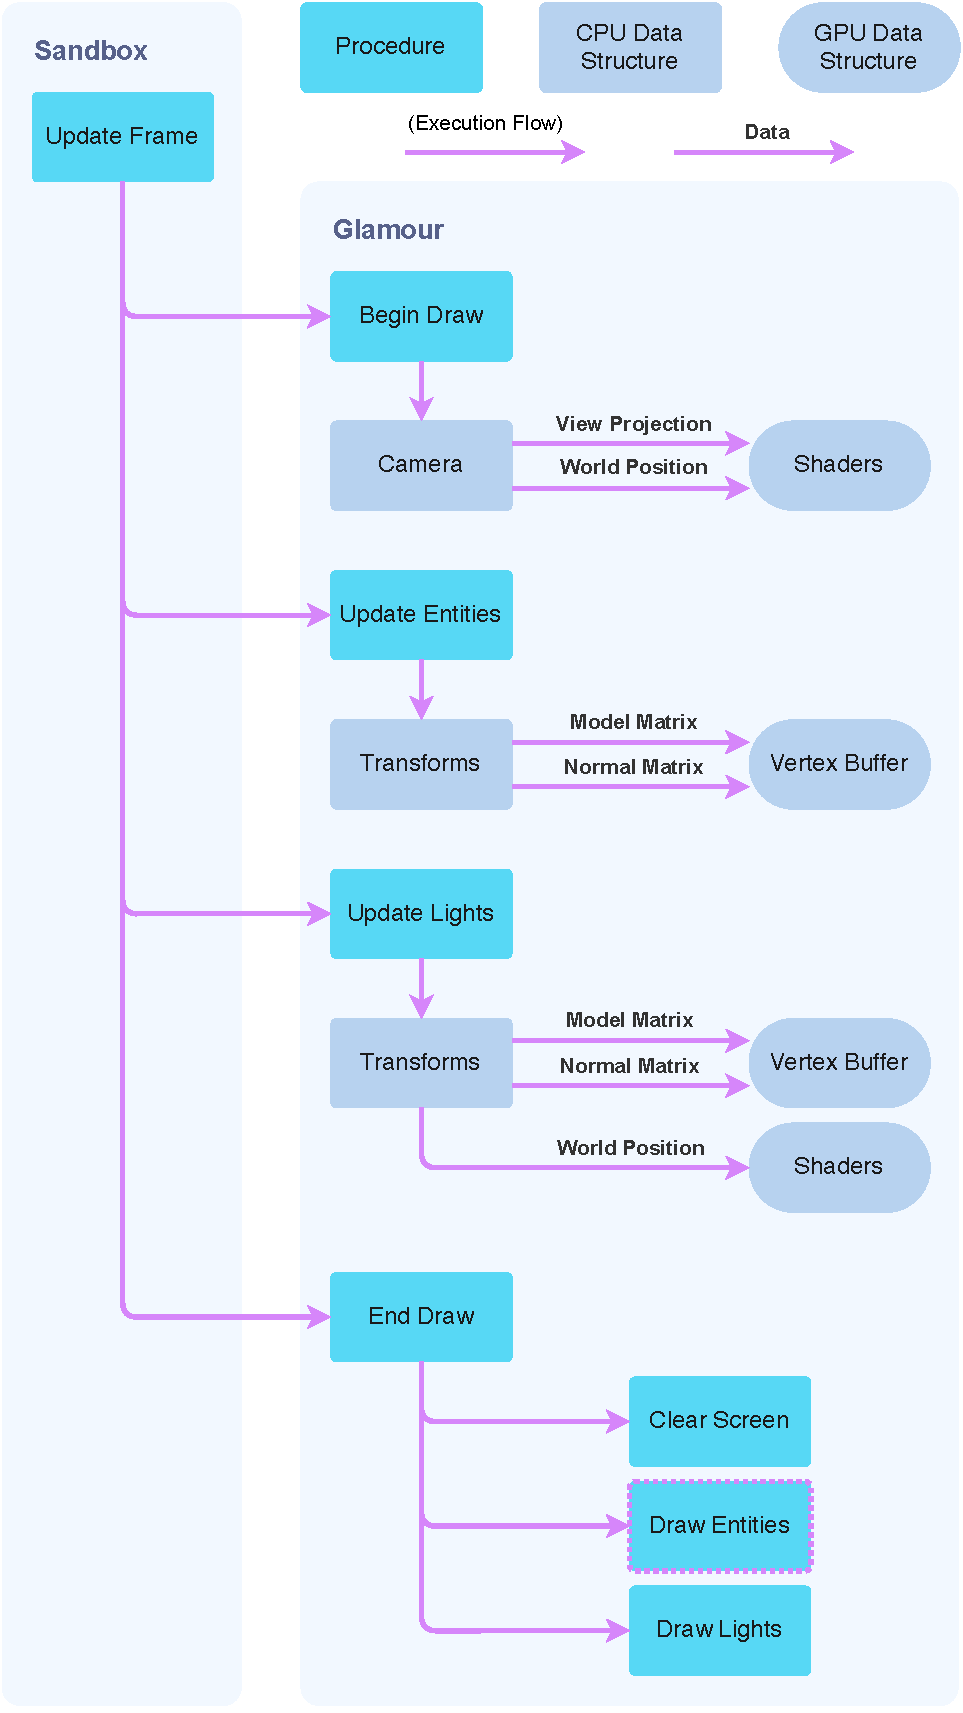
\includegraphics[width=0.7\columnwidth]{../rendering-pipeline.pdf}
  \end{center}
  \caption[Rendering pipeline]{
    \emph{
      The general rendering pipeline.
      \code{Draw Entities} is where the difference between forward and deferred is managed.
    }
  }\label{fig:rendering-pipeline}
\end{figure}

The rendering code almost exactly reflects the \textbf{End Draw} flow:
% \begin{noindent}
  \begin{rustcode}
pub fn end_draw(&mut self) {
    self.clear();
    if self.deferred {
        self.draw_cubes_deferred();
    } else {
        self.draw_cubes_forward();
    }
    self.draw_lights();
}
  \end{rustcode}
% \end{noindent}

The follow sections describe the implementation differences of forward and deferred.
Further explanation of the theory behind forward and deferred can be found at an online article\autocite{owens_forward_2013}.

\subsubsection{Forward}
Forward rendering draws the cubes in a single pass to the default frame buffer.
The vertex shader transforms the vertices and outputs fragment positions, normal directions, and texture coordinates.
The fragment shader receives those parameters along with the details of each light to calculate the shading for every fragment.

After drawing, the depth test throws away fragments that are not visible.

In Appendix~\ref{app:draw-cubes-forward}, some code for forward rendering is explained with comments.

\subsubsection{Deferred}
Deferred rendering is a two-step process consisting of the geometry pass and the lighting pass.

\paragraph{Geometry Pass.}
This pass uses a \emph{Geometry Buffer}, which is a collection of \emph{Frame Buffers} (which are textures) to hold the exact information output by the vertex shader; the same vertex shader used in forward rendering.

After drawing, the depth test throws away fragments that are not visible.

\paragraph{Lighting Pass.}
This pass takes those \emph{Frame Buffers} and uses the information stored in them to calculate the shading.
The lighting calculation is exactly the same as in forward rendering, with the only difference being the parameters come from the textures and not the vertex shader.

The final image is then projected onto on a quad that covers the entire screen and depth information from the geometry pass is copied back to the default depth buffer, so that other objects can be rendered with correct depth testing, e.g., the light cubes, which are always forward rendered.\\

In Appendix~\ref{app:draw-cubes-deferred}, some code for deferred rendering is explained with comments.

\subsection{OpenGL}
% abstracting OpenGL and error handling, \code{gl_call}.

The \code{gl} crate does not provide a safe wrapper around the OpenGL API, it just loads the function pointers into Rust functions.
It is tedious to wrap every OpenGL function call with an \rust{unsafe} block, and that doesn't account for error handling either.
Since this application supports OpenGL 4.1 and above, the error handling is particularly annoying to use.

To package these issues into a flexible solution, Rust's extensive macro system was used.
The \rust{gl_call!()} macro exists to wrap the function in an \rust{unsafe} block, and, if in debug mode, \rust{panic!} (crash) if there are any errors.
OpenGL functions are now all wrapped with this macro, for example, \rust{gl_call!(gl::GenBuffers(1, &mut id));}.
Appendix~\ref{app:gl-call} contains the macro code.

\subsection{MVP Transforms}

\subsubsection{Transform}
The \emph{Coordinate Systems} page on Learn OpenGL\autocite{de_vries_learn_2020} explains the process of MVP (Model-View-Projection) matrices to transform vertices into a space that can be rendered in the OpenGL viewport.

On the usability side, a structure to contain the position, rotation, and scale was required to easily transform entities and reduce the number of matrix multiplications.
% \begin{noindent}
  \begin{rustcode}
struct Transform {
    position: glm::Vec3,
    rotation: glm::Quat,
    scale: glm::Vec3,
}
  \end{rustcode}
  % \end{noindent}
To avoid more matrix transformations, this time on GPU, the \emph{Model Matrix} and its \emph{Normal Matrix} are constructed from the Transform struct CPU side, then sent to the GPU\@.

Sending the position, rotation, and scale to the GPU individually and constructing the matrix there would incur a cost to performance, as that would calculate for every vertex, even though the matrix is the same for all vertices in the mesh.

\subsubsection{Camera}
% \begin{noindent}
  \begin{rustcode}
struct Camera {
    position: glm::Vec3,
    target: glm::Vec3,
    fov: f32,
    aspect: f32,
}
  \end{rustcode}
  % \end{noindent}

The Camera is another basic structure used by the coordinate system.
Using the \code{position} and \code{target}, the view matrix can be calculated, and used to transform vertices relative to the camera.
Using the \code{aspect} and \code{fov}, the projection matrix can be calculated, and used to transform vertices relative to OpenGL's clip-space\autocite{de_vries_learn_2020}.
OpenGL then handles transforming from that clip-space into screen-space.


\subsection{Shaders}

\subsubsection{Shader Builder}
A common pattern in Rust is the \emph{Builder Pattern}.
This is particularly useful for creating shader programs as any number and type of uniform can be specified for the shader, before actually creating the shaders and program on the GPU.
Calling \rust{build()} is what processes all the inputs and returns the shader program object for use.
% \begin{noindent}
  \begin{rustcode}
let shader_lit_for = ShaderBuilder::new(
    include_str!("shaders/lit_for.vert"),
    include_str!("shaders/lit_for.frag"),
)
.with_float4("u_color", glm::vec4(1.0, 1.0, 1.0, 1.0))
.build();
  \end{rustcode}
% \end{noindent}

\subsubsection{Forward v Deferred}
There are a total of eight shaders used in the rendering pipeline.
\begin{itemize}
  \item \code{lit_for.vert} \textbf{Lit Forward Vertex Shader} takes vertex data and outputs fragment position, normal direction, and texture coordinates
  \item \code{lit_for.frag} \textbf{Lit Forward Fragment Shader} takes the output above and every light's data to calculate the shading for the fragment
  \item \code{lit_def_geo.vert} \textbf{Lit Deferred Geometry Pass Vertex Shader} is exactly the same as \code{lit_for.vert}
  \item \code{lit_def_geo.frag} \textbf{Lit Deferred Geometry Pass Fragment Shader} takes the output above and simply outputs it again to be captured by the geometry buffer
  \item \code{lit_def_light.vert} \textbf{Lit Deferred Lighting Pass Vertex Shader} provides texture coordinates of the screen-space quad to the following shader
  \item \code{lit_def_light.frag} \textbf{Lit Deferred Lighting Pass Fragment Shader} almost the same as \code{lit_for.frag} except its inputs come form the geometry buffer
  \item \code{unlit_for.vert} \textbf{Unlit Forward Vertex Shader} merely transforms vertices for the following fragment shader
  \item \code{unlit_for.frag} \textbf{Unlit Forward Fragment Shader} just outputs a flat colour (used for rendering the lights).
\end{itemize}

\subsection{Vertex Arrays}
TODO: uses of VertBasic and VertTrans

\section{Assets}

\subsection{Asset Management}
Since Cargo only deals with code, a \code{build.rs} script was created to facilitate copying the assets source folder to its destination directory relative to the built executable.

There also exists an \code{asset} module that exports a helper function \code{assets_path()} to obtain the assets directory at runtime, to make loading the assets easier.

\subsection{Including resources}
Some files are loaded directly into the application binary at compile time.
This includes the imgui font and the shaders.
Rust has a couple of helper macros that make this trivial, namely, \code{include_bytes!()} and \code{include_str!()}.

This is something that seems incredibly simple, but cannot be done with just C++ without changing the original file to make it a raw string.
\emph{50 points to \textbf{Rust}lepuff!}

\section{Data Collection}

TODO: Details on how data is collected.

\section{Code Quality}

\subsection{Tests}
The Rust tool-chain comes with built in testing and documentation tool, they can even be combined.
Now, there are not a lot of tests in source code at the time of writing, as a lot of it is OpenGL code, which is notoriously hard to ensure robustness because of the multitude of versions and implementations.

However, a few test experiments were completed as part of a bit of documentation, as rust will compile doc-comment example code and run it as integration tests.

\subsection{Documentation}
There also is not a lot of source code documentation available, but Cargo can generate API documentation from the source code into a web page.

So, when code is pushed to the GitHub repository, it is built, tested, and the documentation is generated and put up on this website \url{https://glamour.davidjh.com/doc/glamour/index.html}.

\subsection{Benchmarks}
Cargo has benchmark tests in nightly preview at the moment, but the \code{criterion} crate exists to aid in benchmarking functions in the meantime.

The benchmarks run a some arbitrary code a bunch of times — generally thousands — and takes a sample of those to compare to the previous run, so the developer can track performance trends.

These benchmarks have been used to improve the performance of the \code{Transform} matrix calculation (which runs thousands of times a frame), and confirm where multi-threading improves performance (mainly by paralleling all those matrix transformations).

\section{Future Work}

TODO: Details on issues and improvements that should be addressed, and speculate about other uses for the software.

\begin{itemize}
  \item Graphics API abstraction, could port to Vulkan/Metal/DirectX/OpenGL-ES
  \item OS Platform abstraction (maybe. glutin/winit handles a lot of that)
  \item Separate window/rendering thread
  \item Vertex Arrays have a lot of nonsense hard coded stuff
  \item G-buffer/frame-buffers could do with a refactor
  \item Shaders should be loaded from disk
  \item Add actual docs, tests, and benchmarks
  \item Once this is an acceptable renderer, I might add more game engine features. Maybe try and make a small game
\end{itemize}

\newpage

%----------------------------------------------------------------------------------------
%	BIBLIOGRAPHY
%----------------------------------------------------------------------------------------

\printbibliography[heading=bibintoc]{}

\newpage

%----------------------------------------------------------------------------------------
%	APPENDICES
%----------------------------------------------------------------------------------------

\begin{appendices}
  \section{Sandbox Main Function}\label{app:sandbox-main}
  % \begin{noindent}
  \begin{rustcode}
fn main() {
    let mut app = glamour::App::new("Glamour Sandbox", 1920, 1080);
    let sandbox_layer = SandboxLayer::new("SandboxLayer");
    app.push_layer(Box::new(sandbox_layer));
    app.run();
}
  \end{rustcode}
  % \end{noindent}

  \section{Draw Cubes Forward}\label{app:draw-cubes-forward}
  % \begin{noindent}
  \begin{rustcode}
fn draw_cubes_forward(&self) {
    // send transform data (position, rotation, scale) to the GPU
    self.cube_trans_vbo.set_data();
    // select the lit shader for forward rendering
    self.lit_for_shader.bind();
    // select the cube texture
    self.cube_tex.bind();
    // select the cube vertices
    self.cube_vao.bind();
    // draw an instance of the cube vertices for every transform
    gl_call!(gl::DrawElementsInstanced(
        gl::TRIANGLES,
        self.cube_vao.index_buf().len() as i32,
        gl::UNSIGNED_INT,
        std::ptr::null(),
        self.cube_trans_vbo.vertices().len() as i32,
    ));
    // deselect everything
    self.cube_vao.unbind();
    self.cube_tex.unbind();
    self.cube_shader.unbind();
}
  \end{rustcode}
  % \end{noindent}

  \section{Draw Cubes Deferred}\label{app:draw-cubes-deferred}
  % \begin{noindent}
  \begin{rustcode}
fn draw_cubes_deferred(&self) {
    // send transform data (position, rotation, scale) to the GPU
    self.cube_trans_vbo.set_data();

    // goemetry pass (must be cleared black beforehand)
    // select geometry buffer to render to
    self.g_buf.bind();
    {
        gl_call!(gl::Clear(gl::COLOR_BUFFER_BIT | gl::DEPTH_BUFFER_BIT));
        // select the geometry lit shader for deferred rendering
        self.lit_def_geo.bind();
        // select the cube texture
        self.cube_tex.bind();
        // select the cube vertices
        self.cube_vao.bind();
        // draw an instance of the cube vertices for every transform
        gl_call!(gl::DrawElementsInstanced(
            gl::TRIANGLES,
            self.cube_vao.index_buf().len() as i32,
            gl::UNSIGNED_INT,
            std::ptr::null(),
            self.cube_trans_vbo.vertices().len() as i32,
        ));
        // deselect everything
        self.cube_vao.unbind();
        self.cube_tex.unbind();
        self.lit_def_geo.unbind();
    }
    self.g_buf.unbind();

    // lighting pass
    gl_call!(gl::Clear(gl::COLOR_BUFFER_BIT | gl::DEPTH_BUFFER_BIT));
    {
        // select the lighting lit shader for deferred rendering
        self.lit_def_light.bind();
        // select the frame buffers from the geometry buffer
        self.g_buf.bind_bufs();
        // select quad vertices to cover the screen
        self.ndc_quad_vao.bind();
        // draw the screen quad
        gl_call!(gl::DrawArrays(gl::TRIANGLE_STRIP, 0, 4));
        // deselect everything
        self.ndc_quad_vao.unbind();
        self.g_buf.unbind_bufs();
        self.lit_def_light.unbind();
    }

    // blit depth buffer (so lights can be depth tested correctly)
    self.g_buf.blit_depth();
}
  \end{rustcode}
  % \end{noindent}

  \section{\code{gl_call!}}\label{app:gl-call}
  % \begin{noindent}
    \begin{rustcode}
#[macro_export]
macro_rules! gl_call {
    ($gl_fn:expr) => {{
        let result = unsafe { $gl_fn };
        if cfg!(debug_assertions) {
            let errors = $crate::gl_call::gl_get_errors();
            if !errors.is_empty() {
                panic!(
                    "OpenGL Errors: {}",
                    errors
                        .iter()
                        .map($crate::gl_call::gl_get_error_name)
                        .collect::<Vec<_>>()
                        .join(", ")
                );
            }
        }
        result
    }};
}
    \end{rustcode}
    % \end{noindent}

\end{appendices}

\end{document}
